\chapter {Introduction}

Implicit Bias is one of the many problems that the developer needs to be aware of when training an optimization model. Most algorithms, such as gradient descent optimization, do not contain implicit bias within. Instead, the implicit bias of the algorithm starts to appear during the training phase of the data. During the training epochs, the model will start to pick up certain features within the dataset that, while prevalent over the training set, may not apply to other training data in general.
 
Implicit bias in optimization is a problem because it can lead to models that are biased towards certain features or patterns in the data. This bias can lead to poor generalization performance and may also perpetuate or amplify existing biases in the data. In particular, when the training data is itself biased or limited in some way, the resulting model can inherit these biases and make unfair or incorrect predictions on new, unseen data. This also has serious consequences, where the predictions of the model may favor one class of the data over the other.

While avoiding implicit bias within the training dataset is impossible due to its cause, we can still attempt to reduce or minimize the negative impacts that the implicit bias may have on our training model. For instance, do we still benefit from implicit regularization when minimizing the logistic loss on separable data? While it is clear that the norm of the predictor itself is not minimized, since it grows to infinity, for prediction, only the direction of the predictor, i.e. the normalized $w(t)/ ||w(t)||$ , is important. How does $w(t)/ ||w(t)||$ behave as $t \rightarrow +\infty$ when we minimize the logistic (or similar) loss using gradient descent on separable data, i.e., when it is possible to get zero misclassification error and thus drive the loss to zero?

Overall, implicit bias in gradient descent can have significant negative consequences, particularly when it leads to unfair or discriminatory outcomes. It's important for machine learning practitioners to be aware of these issues and take steps to address them, such as by using diverse training data, testing for biases in the data, and using debiasing algorithms.

\chapter{Related Work and Novelty}

\section{Related Work}

The paper we selected for the research, “The Implicit Bias of Gradient Descent on Separable Data”, introduced various methods of gradient descent and compared the implicit biases between each of the models to show the accuracy of their results.

In this paper, the authors examine gradient descent on unregularized logistic regression problems, with homogeneous linear predictors on linearly separable datasets. We show the predictor converges to the direction of the max-margin (hard margin SVM) solution. The result also generalizes to other monotone decreasing loss functions with an infimum at infinity, to multi-class problems, and to training a weight layer in a deep network in a certain restricted setting.\cite{1} Furthermore, we show this convergence is very slow, and only logarithmic in the convergence of the loss itself. This can help explain the benefit of continuing to optimize the logistic or cross-entropy loss even after the training error is zero and the training loss is extremely small, and, as we show, even if the validation loss increases. Our methodology can also aid in understanding implicit regularization in more complex models and with other optimization methods.

The shortcoming of this paper that we have observed is that the paper only considered the implicit bias caused by training data on traditional stochastic gradient descent. While the paper provide sufficient proof to its thesis and statements, we would like to learn more whether we can reduce the negative influence of the implicit bias by trying out different gradient optimization method or modifying the current one to prevent the training algorithm from using irrelevant data features to train its model.

\section{Novelty}

For our research, we intend to implement another gradient algorithm that we had learned from the class, and compare its results to determine the implicit biases between the gradient descent algorithms.

We will implement a new algorithm, Adaptive Moment Estimation(ADAM). ADAM is an extension of the gradient descent algorithm, specifically the stochastic gradient descent algorithm. ADAM combines two stochastic gradient descent approaches, Adaptive Gradients, and Root Mean Square Propagation. Instead of using the entire data set to calculate the actual gradient, this optimization algorithm uses a randomly selected data subset to create a stochastic approximation.

Unlike the traditional stochastic gradient descent, which maintains a constant learning rate during the training phase, ADAM is able to adjust its learning rate based on the training data. When processing a large quantity of data, the training result by stochastic gradient descent algorithms may take longer to converge, since it may encounter multiple local minima within a dataset. Adaptive Moment Estimation, on the other hand, facilitates the computation of learning rates for each parameter using the first and second moment of the gradient, thus improving the computation efficiency of the algorithm, and requiring less memory to perform than other methods. 

\chapter{Methods}

% \begin{align*}\label{2}
\section{Algorithm}

\subsection{Average Stochastic Gradient Descent \ (ASGD)}
In addition to SGD used in the paper, we try to implement ASGD to test its performance. Based on SGD, we will take the mean value of the result as our final solution in ASGD. So for the regular Stochastic Gradient Descent $ w_{t+1} = w_t - \tau \nabla f(w_t) $, we simply take the mean value of $ \overline{w} = \frac{1}{N} \sum_{t=1}^{N} w_t $ to reduce the impact of noise. So it might be more effective if the data is influenced by noise.

\subsection{Adaptive Moment Estimation\ (ADAM)}
We implement the ADAM optimization algorithm to resolve the problem mentioned above. Unlike stochastic gradient descent, the adaptive moment estimation method requires only the first and second gradients to update the weight and step size during the training phase. 

In addition to using a new training function, we also implemented a linear regulator function to compensate for the implicit bias caused by the algorithm. This can help to reduce the impact of features that are less relevant to the task at hand and can reduce the impact of any biases in the data. There are two approaches to dealing with the implicit bias caused by training data with the optimizing model: the first approach is the increase the regulation weights, which can help to compensate for any potential bias or deviation during each epoch of training, the second approach is the decrease the weight decay of the model, which can help to eliminate the potential training bias caused by introducing irrelevant data feature to the training of the model. 

The learning rate parameter $(lr)$ is a hyper-parameter that determines the step size taken during the optimization process in machine learning models. It can have an important influence on the implicit bias of the model. A high learning rate can lead to a more aggressive optimization process, where the weights of the model are updated quickly in response to the gradients of the loss function. This can lead to a model that overfits the training data and has high variance. In this case, the model may be biased towards the specific features and patterns in the training data, which can lead to poor generalization performance on new, unseen data.\cite{2}

On the other hand, a low learning rate can lead to a slower optimization process, where the weights of the model are updated more gradually in response to the gradients of the loss function. This can lead to a model that is biased towards simpler and more general patterns in the data, which can improve its ability to generalize to new, unseen data. However, if the learning rate is too low, the optimization process may be too slow and the model may not converge to an optimal solution. 

Therefore, the choice of the learning rate can have an important influence on the implicit bias of the model. A carefully chosen learning rate can help to balance the trade-off between bias and variance in the model and improve its generalization performance. In practice, the optimal learning rate depends on the specific problem and the nature of the data, and it often needs to be tuned through experimentation.

Reducing weight decay can reduce implicit bias in optimization methods because it allows the model to learn more complex and diverse representations of the data. When the weight decay is high, the model is encouraged to have smaller weights, which can lead to a simpler model that is biased towards a certain set of features or patterns in the data. This bias can be problematic when the training data is itself biased or limited in some way, as it can lead to a model that is over-reliant on certain features and performs poorly on new, unseen data.\cite{3}

By reducing weight decay, the model is allowed to have larger weights, which can lead to a more complex and diverse set of representations. This can help to reduce bias in the model and improve its ability to generalize to new data. In particular, reducing weight decay can be useful when dealing with biased data or in cases where there is a large amount of variation in the data that the model needs to capture.\cite{4} However, we need to balance the use of weight decay with other regularization techniques and carefully tune the hyper-parameters to achieve optimal performance.

The Pseudo-code for implementing the ADAM algorithm is listed below:

\begin{eqnarray}
    && \textbf{input}: \gamma(lr),\ \beta_1,\ \beta_2(betas),\ \theta_0(params),\ f(\theta)(objective),\  \nonumber \\
    && \qquad \quad \ \lambda(weight decay),\ amsgrad,\ maximize \nonumber \\
    && \textbf{initialize}: m_0 \leftarrow 0\ (first\ moment), v_0 \leftarrow 0\ (second\ moment), \hat{v_0}^{max} \leftarrow 0  \nonumber \\
    && \textbf{for}\ t=1\ to \cdots do \nonumber \\ 
    && \quad \textbf{if}\ maximize: \nonumber \\ 
    && \quad \quad  g_t \leftarrow -\nabla_\theta f_t(\theta_{t-1}) \nonumber \\ 
    && \quad \textbf{else}: \nonumber \\ 
    && \quad \quad  g_t \leftarrow \nabla_\theta f_t(\theta_{t-1}) \nonumber \\ 
    && \quad \textbf{if}\ \lambda \neq 0: \nonumber \\ 
    && \quad \quad  g_t \leftarrow g_t + \lambda \theta_{t-1} \nonumber \\ 
    && \quad  m_t \leftarrow \beta_1 m_{t-1} + (1-\beta_1)g_t  \nonumber \\ 
    && \quad  v_t \leftarrow \beta_2 v_{t-1} + (1-\beta_2)g_t^2  \nonumber \\ 
    && \quad  \hat{m_t} \leftarrow m_t / (1-\beta_1^t)  \nonumber \\ 
    && \quad  \hat{v_t} \leftarrow v_t / (1-\beta_2^t)  \nonumber \\ 
    && \quad \textbf{if}\ amsgrad: \nonumber \\ 
    && \quad \quad \hat{v_0}^{max} \leftarrow max(\hat{v_0}^{max}, \hat{v_0}) \nonumber \\ 
    && \quad \quad \theta_t \leftarrow \theta_{t-1} - \gamma \hat{m_t} /(\sqrt{\hat{v_t}^{max}} + \epsilon) \nonumber \\ 
    && \quad \textbf{else}: \nonumber \\ 
    && \quad \quad \theta_t \leftarrow \theta_{t-1} - \gamma \hat{m_t} /(\sqrt{\hat{v_t}} + \epsilon) \nonumber \\ 
    && \textbf{return} \ \theta_t \nonumber \\ 
\end{eqnarray}

\subsection{Adam with weight decay\ (AdamW)}

Apart from the ADAM optimization algorithm, we also use AdamW to solve the problem. Based on ADAM, AdamW uses a weight decay to renew the result. In the last step in ADAM, we add a decay as $w \theta_{t-1} $ to overfit less and generalize better. The rate of the weight decay per step $w$ defines the relative importance of minimizing the original loss function (more important if small $w$ is chosen) and finding small weights( more important if large $w$ is chosen).

The Pseudo-code for the AdamW algorithm is listed below, bolding the difference from ADAM.

\begin{eqnarray}
    && \textbf{input}: \gamma(lr),\ \beta_1,\ \beta_2(betas),\ \theta_0(params),\ f(\theta)(objective),\  \nonumber \\
    && \qquad \quad \ \lambda(weight decay),\ amsgrad,\ maximize \nonumber \\
    && \textbf{initialize}: m_0 \leftarrow 0\ (first\ moment), v_0 \leftarrow 0\ (second\ moment), \hat{v_0}^{max} \leftarrow 0  \nonumber \\
    && \textbf{for}\ t=1\ to \cdots do \nonumber \\ 
    && \quad \textbf{if}\ maximize: \nonumber \\ 
    && \quad \quad  g_t \leftarrow -\nabla_\theta f_t(\theta_{t-1}) \nonumber \\ 
    && \quad \textbf{else}: \nonumber \\ 
    && \quad \quad  g_t \leftarrow \nabla_\theta f_t(\theta_{t-1}) \nonumber \\ 
    && \quad \textbf{if}\ \lambda \neq 0: \nonumber \\ 
    && \quad \quad  g_t \leftarrow g_t + \lambda \theta_{t-1} \nonumber \\ 
    && \quad  m_t \leftarrow \beta_1 m_{t-1} + (1-\beta_1)g_t  \nonumber \\ 
    && \quad  v_t \leftarrow \beta_2 v_{t-1} + (1-\beta_2)g_t^2  \nonumber \\ 
    && \quad  \hat{m_t} \leftarrow m_t / (1-\beta_1^t)  \nonumber \\ 
    && \quad  \hat{v_t} \leftarrow v_t / (1-\beta_2^t)  \nonumber \\ 
    && \quad \textbf{if}\ amsgrad: \nonumber \\ 
    && \quad \quad \hat{v_0}^{max} \leftarrow max(\hat{v_0}^{max}, \hat{v_0}) \nonumber \\ 
    && \quad \quad \theta_t \leftarrow \theta_{t-1} - \gamma ( \hat{m_t} /(\sqrt{\hat{v_t}^{max}} + \epsilon) + \boldsymbol{w \theta_{t-1}} )\nonumber \\ 
    && \quad \textbf{else}: \nonumber \\ 
    && \quad \quad \theta_t \leftarrow \theta_{t-1} - \gamma (\hat{m_t} /(\sqrt{\hat{v_t}} + \epsilon) + \boldsymbol{w \theta_{t-1}} ) \nonumber \\ 
    && \textbf{return} \ \theta_t \nonumber \\ 
\end{eqnarray}

\section{Dataset}

For the dataset, we used The CIFAR-10 dataset. The dataset is divided into five training batches and one test batch, each with 10000 images. The test batch contains exactly 1000 randomly-selected images from each class. The training batches contain the remaining images in random order, but some training batches may contain more images from one class than another. Between them, the training batches contain exactly 5000 images from each class.

We will use this data set to train the optimization model that we designed, and observe its performance in accuracy, precision, as well as assess its implicit bias as it went through more training epochs.

\section{Experiment}

For this experiment, we will test the performance of the Adam algorithm in various learning rates and weight decay parameters. For each trial, we will run for about 100 epochs. The training and validation data that we are using are two classes of CIFAR data: 1s and 5s. For each epoch, we will measure the training loss, validation loss, and error for both classes of data.

\chapter{Evaluation}
\section{Stochastic Gradient Descent}
Firstly, we implemented the original code from the paper and got the results using the SGD method. We tested two classes of CIFAR data as 1s and 5s. Figure 4.1 shows the rate of training error and validation error, with the learning rate of 1e-3 and 50 epochs of training. From the graph, we can find that the converging validation rate is higher than that of the training rate, which is expected.

\begin{figure}[H]
    \centering % figure is centered on the page
        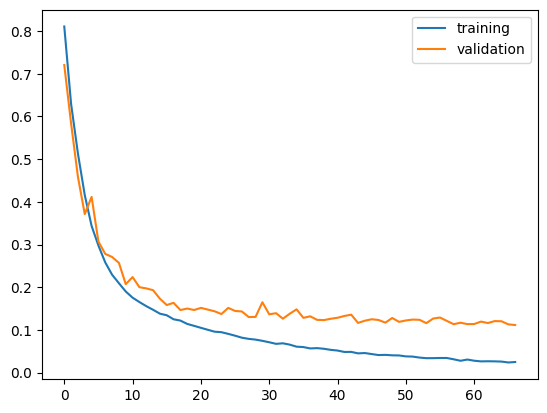
\includegraphics[width=0.6\linewidth]{./SGD.png} 
    \caption{Training error and Validation error of SGD.}
\end{figure}

Figure 4.2 shows the L2 norm of the SGD. We observed that L2 norm increases when iteration increases.

\begin{figure}[H]
    \centering % figure is centered on the page
        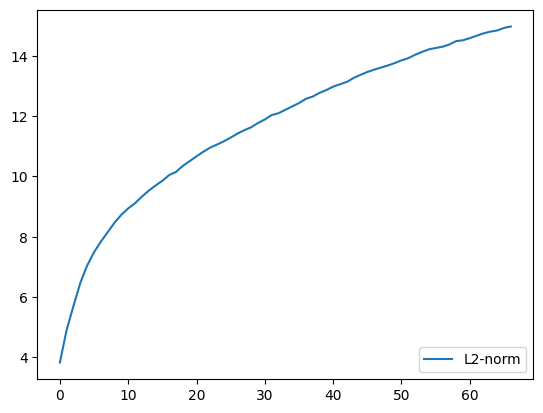
\includegraphics[width=0.6\linewidth]{./SGDl2.png} 
    \caption{L2-norm of SGD.}
\end{figure}

\section{Averaged Stochastic Gradient Descent}

We implemented ASGD to the data set, testing two classes of CIFAR data for 1s and 5s. Figure 4.3 shows the rate of training error and validation error, with the learning rate of 1e-3 and 50 epochs of training. Compared with the above figure of SGD, we can see that the converging training and validation error for the ASGD algorithm is lower than that of the SGD algorithm. If the noise of the data increases, the difference will be larger.

\begin{figure}[H]
    \centering % figure is centered on the page
        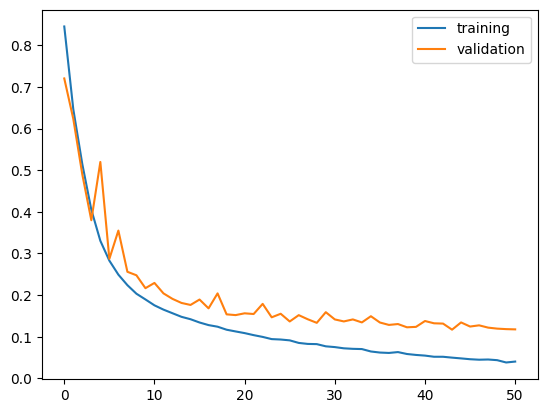
\includegraphics[width=0.6\linewidth]{./ASGD.png} 
    \caption{Training error and Validation error of ASGD.}
\end{figure}

Figure 4.4 shows the L2 norm of the ASGD. It has the same trend but a slower increase than that of SGD.

\begin{figure}[H]
    \centering % figure is centered on the page
        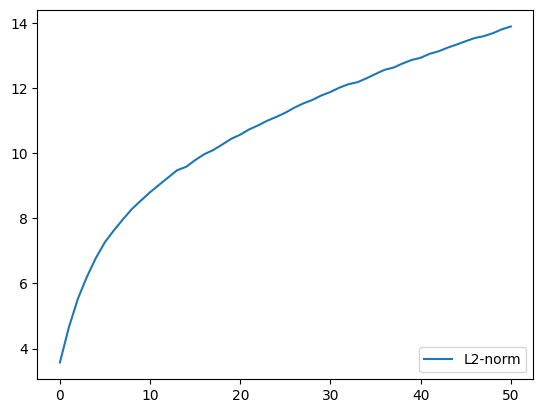
\includegraphics[width=0.6\linewidth]{./ASGDl2.png} 
    \caption{L2-norm of ASGD.}
\end{figure}

\section{Adam}
We used Adaptive Moment Estimation\ (ADAM) for our training, with a learning rate of 1e-3 and 50 epochs of training. Figure 4.5 shows the rate of training error and validation error, for training 50 epochs. From the graph, we found that the trend of convergence is faster than SGD and ASGD methods, since it comes to a smaller error rate in the same iterations and training epochs.

\begin{figure}[H]
    \centering % figure is centered on the page
        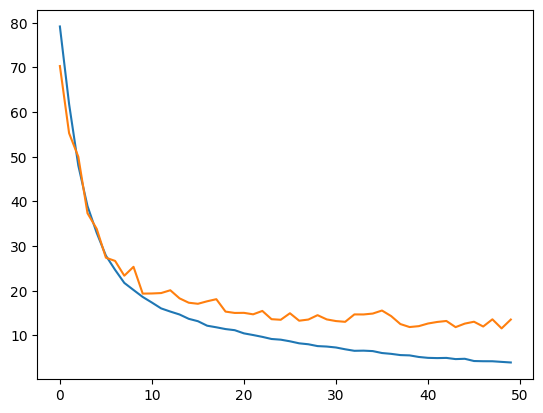
\includegraphics[width=0.6\linewidth]{./ADAM.png} 
    \caption{Training error and Validation error of Adam.}
\end{figure}

We also drew the L2 norm of ADAM, shown in Figure 4.6. From Figure 4.6, we observed that it has the same trend as SGD and ASGD, which is as iteration increases, the L2 norm increases.

\begin{figure}[H]
    \centering % figure is centered on the page
        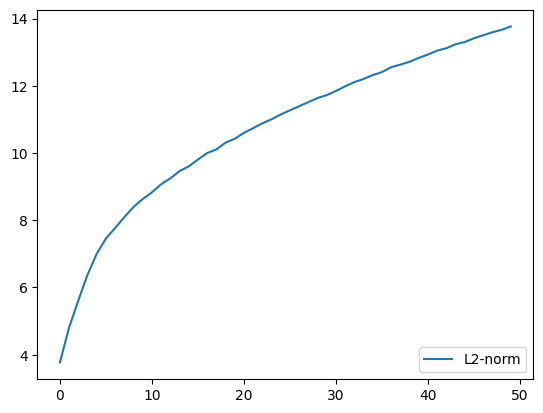
\includegraphics[width=0.6\linewidth]{./ADAMl2.png} 
    \caption{L2-norm of Adam.}
\end{figure}


\section{AdamW}
We also used AdamW for our training, with a learning rate of 1e-3 and 50 epochs of training. Figure 4.7 shows the rate of training error and validation error. Compared with the above figure of Adam, we can find that the validation error converges better at last.
\begin{figure}[H]
    \centering % figure is centered on the page
        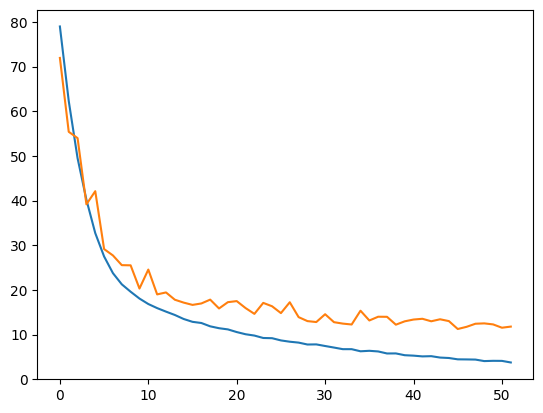
\includegraphics[width=0.6\linewidth]{./ADAMW.png} 
    \caption{Training error and Validation error AdamW.}
\end{figure}

Figure 4.8 shows the L2 norm of Adamw.

\begin{figure}[H]
    \centering % figure is centered on the page
        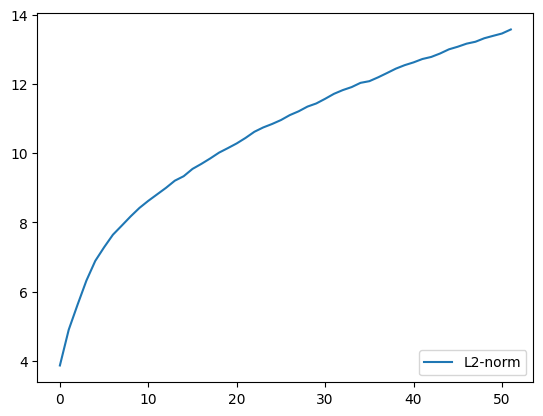
\includegraphics[width=0.6\linewidth]{./ADAMWl2.png} 
    \caption{L2-norm of AdamW.}
\end{figure}

\chapter{Conclusion}

\section{Summary}
In our comparison between the SGD and ASGD, we can observe that the converging value of the training and validation error for the ASGD algorithm is lower than that of the SGD algorithm. This result is to be expected since the ASGD.

For Adam and weighted Adam algorithms, we can see a similar trend in the output. However, the convergence rate of the training and validation error is faster than that of the SGD pairs, where it converges to the same training and validation error value within short iterations and training epochs. We also observed that as the training epoch increases, the L2 norm, or regularization norm, also increases. This shows that the implicit bias of the algorithms increases as the model goes through more training iterations. By comparing the L2 norms, we can conclude that the Adam algorithm has a slower increase of L2 norm than that of SGD, thus proving that Adam model can reduce the implicit bias caused by the training dataset. Since the Adam algorithm uses a smaller learning rate than that of SGD (where $lr = 0.1$), we can infer that a smaller learning rate of the model can reduce the implicit bias caused by training data.

The limitations of our research is that despite signs of differences exist in both training and validation error for each training algorithm, the algorithms that we had implemented are homogenous, since Adam algorithm is derived from the stochastic gradient descent algorithm. In addition, the training algorithms that we are currently testing on a small number of classes. While the results and performance on these classes showed promising results, we have yet to push the testing of the algorithm to a wider range of images or dataset.

\section{Future Work}
For our future work, we will be focusing on three aspects as the extension of our current work. First, we will attempt to substantiate our conclusion with a dataset of greater quantities and varieties, which will allow us to discover a more standardized approach to reduce the implicit bias during the training process of the data. Second, we also plan to explore optimization methods other than simple gradient descent, and designing an algorithm of our own that can perfect the gradient descent algorithm to reduce the influence caused by implicit bias. 

\chapter{Acknowledgements}

This report is done by both authors with tasks being shared in an equal fashion. Shuohui is in charge of both designing and running the training model and visualizing the data structure, while Yujie is primarily in charge of research for novel algorithms and providing ideas for the project.

\bibliography{References.bib}
% \begin{thebibliography}{9}
% \bibitem{soudry2022implicit}
% @misc{soudry2022implicit,
%       title={The Implicit Bias of Gradient Descent on Separable Data}, 
%       author={Daniel Soudry and Elad Hoffer and Mor Shpigel Nacson and Suriya Gunasekar and Nathan Srebro},
%       year={2022},
%       eprint={1710.10345},
%       archivePrefix={arXiv},
%       primaryClass={stat.ML}
% }
% \bibitem{2020implicit}
% @misc{gunasekar2020characterizing,
%       title={Characterizing Implicit Bias in Terms of Optimization Geometry}, 
%       author={Suriya Gunasekar and Jason Lee and Daniel Soudry and Nathan Srebro},
%       year={2020},
%       eprint={1802.08246},
%       archivePrefix={arXiv},
%       primaryClass={stat.ML}
% }
% \bibitem{schliserman2022stability}
% @misc{
%       title={Stability vs Implicit Bias of Gradient Methods on Separable Data and Beyond}, 
%       author={Matan Schliserman and Tomer Koren},
%       year={2022},
%       eprint={2202.13441},
%       archivePrefix={arXiv},
%       primaryClass={cs.LG}
% }

% \bibitem{jin2023implicit}
% @misc{jin2023implicit,
%       title={Implicit Bias of Gradient Descent for Mean Squared Error Regression with Two-Layer Wide Neural Networks}, 
%       author={Hui Jin and Guido Montúfar},
%       year={2023},
%       eprint={2006.07356},
%       archivePrefix={arXiv},
%       primaryClass={stat.ML}
% }
% \end{thebibliography}